\documentclass[dvipdfmx]{beamer}
\usepackage{bxdpx-beamer}% dvipdfmxなので必要
\usepackage{pxjahyper}% 日本語で'しおり'したい
\renewcommand{\kanjifamilydefault}{\gtdefault}% 既定をゴシック体に


%% テーマ
\usetheme{metropolis}           % Use metropolis theme
%% 参照
\def\figref#1{図\ref{#1}}
\def\tblref#1{表\ref{#1}}
\def\eqref#1{式(\ref{#1})}

\newlength{\mytotalwidth}
\mytotalwidth=\dimexpr\linewidth-5mm
\newlength{\mycolumnwidth}
\mycolumnwidth=\dimexpr\mytotalwidth-5mm

\usepackage{graphicx}
\newcommand{\thickhrulefill}{\leavevmode\leaders\hrule depth-1.2pt height 3.2pt\hfill\kern0pt}
\newcommand{\indicatewidth}[1]{\thickhrulefill{#1}\thickhrulefill}
\usepackage{bm}
\usepackage{scalefnt}

\renewcommand{\figurename}{図}
\renewcommand{\tablename}{表}
\setbeamertemplate{caption}[numbered]

%% コンテンツ
\title{Monocular template-based reconstruction of inextensible surfaces  \cite{Perriollat2011}}
\date{\today}
\author{\input{name.tex}}
\institute{}


\begin{document}
  \maketitle
  \section{先週の残り}
  \begin{frame}{SOCP定式化}
    制約条件:再投影誤差=2次錘制約条件
    \begin{equation}
        \| 
        \frac{1}{\mathrm{\bm{p}}_3^{\mathrm{T}} \bm{Q}_i} \left(
        \begin{array}{c}
          \mathrm{\bm{p}}_1^{\mathrm{T}} \bm{Q}_i  \\
          \mathrm{\bm{p}}_2^{\mathrm{T}} \bm{Q}_i
        \end{array}
      \right)
     - \bm{q}_i^{\prime}\| \le \varepsilon_{\mathcal{I}}
     \label{eq:cons_tmp_img}
    \end{equation}

    3次元表面点の深度最大化問題→SOCP定式化可能 \\
    \begin{equation}
        \begin{aligned}
            & \underset{\bm{Q}} {\text{max}} && {\bm{p}}_3^{\mathrm{T}} \sum_{i=1}^{n_c} \bm{Q}\\
        &\text{subject to} &&
            \tiny
            \| 
            \left[
            \begin{array}{c}
              \mathrm{\bm{p}}_1^{\mathrm{T}}  \\
              \mathrm{\bm{p}}_2^{\mathrm{T}}
            \end{array}
            \right] \bm{Q}_i
          - \bm{q}_i^{\prime}\mathrm{\bm{p}}_3^{\mathrm{T}} \bm{Q}_i \| \le \varepsilon_{\mathcal{I}} \mathrm{\bm{p}}_3^{\mathrm{T}} \bm{Q}_i \normalsize &&& \forall i \in \{1, ..., n_c\}\\
        &                  && \| \bm{Q}_i -\bm{Q}_j\| \le d_{ij}  &&& \forall(i, j) \in \varepsilon \\
        &                  && \mathrm{\bm{p}}_3^{\mathrm{T}} \ge 0  &&&  \forall i \in \{1, ..., n_c\}
        \end{aligned}
        \label{eq:socp}
    \end{equation}
  \end{frame}
  \begin{frame}{非伸長性制約条件}
      表面関数$\mathcal{W}$の非伸張性:制約条件$\varepsilon_i(\mathcal{W})$ \\
      特性コスト関数→グリッド点で離散化 \\
      \begin{equation}
          \varepsilon_i(\mathcal{W})=\sum_{j=1}^{n_j}\|\mathrm{J}(\bm{g}_j)^{\mathrm{T}}\mathrm{J}(\bm{g}_j) - \mathrm{I}_2 \|^2
          \label{eq:isometry_orthonormal}
      \end{equation}
      $\{\bm{g}_j\}_{j=1}^{n_j}$:グリッド上の点,$n_j = 30$
  \end{frame}
  \begin{frame}{表面モデルの媒介変数表示}
      媒介変数
      \begin{itemize}
          \item Basis-SplineベースのFFDが使える
          \item Splineの制御点→最適化問題の変数
      \end{itemize}
      モデルの媒介変数表示$\mathcal{W}_{\bm{\ell}}: \mathbb{R}^2 \to \mathbb{R}^3$
      \begin{eqnarray}
          \mathcal{W}_{\bm{\ell}}(\mathrm{\bm{q}}) &=& \sum_{j=0}^{n_u}\sum_{k=0}^{n_v} \bm{\ell}_{jk}N_j(u)N_k(v) \\
          \mathcal{W}_{\bm{\ell}}(\mathrm{\bm{q}}) &=& \mathrm{W}_i\bm{\ell}
      \end{eqnarray}

    $\mathrm{\bm{q}} = (u, v)$:テンプレート画像上の点 \\
    $\bm{\ell}_{jk}; j \in \{0, \dots, n_u\}, k \in \{0, \dots, n_v\}$:3次元点の媒介変数 \\
    $N_{j},N_{k}$:3次の多項式B-spline基底関数 \\
    $\mathrm{W}_i$:点$\mathrm{\bm{q}}_i$にのみ依存する$3\times n_u n_v$の行列

    \begin{itemize}
        \item $\mathcal{W}_{\bm{\ell}}$は線形結合
    \end{itemize}
  \end{frame}
  \begin{frame}{B-Splineの基底関数\cite{Rueckert1999}}
      3次のB-Spline基底関数:$N_j,j\in\{0,\dots,3\}$
      \begin{eqnarray}
          N_0(u) &=& \frac{(1-u)^3}{6} \\
          N_1(u) &=& \frac{(3u^3-6u^2+4)}{6} \\
          N_2(u) &=& \frac{(-3u^3+3u^2+3u+1)}{6} \\
          N_3(u) &=& \frac{u^3}{6}
      \end{eqnarray}
  \end{frame}
  \begin{frame}{最小2乗問題における表面推定}
      \begin{itemize}
          \item \eqref{eq:socp}の3次元点$Q_i$を$\mathrm{W}_i\bm{\ell}$で置き換え
      \end{itemize}
      \eqref{eq:isometry_orthonormal}の媒介変数表示,最小化問題定式化の制約条件
    \begin{equation}
        \left|\left|
        \left( 
            \left[
                \begin{array}{c}
                    \mathrm{\bm{p}}_1^{\mathrm{T}}  \\
                    \mathrm{\bm{p}}_2^{\mathrm{T}}
                \end{array}
            \right]
            - \bm{q}_i^{\prime}\mathrm{\bm{p}}_3^{\mathrm{T}} 
        \right)\mathrm{W}_i\bm{\ell}
        \right|\right|
        \le \varepsilon_{\mathcal{I}}\mathrm{\bm{p}}_3^{\mathrm{T}}\mathrm{W}_i\bm{\ell}
        \label{eq:constraint}
    \end{equation}
  \end{frame}
  \begin{frame}{表面形状の推定}
      \begin{itemize}
          \item \eqref{eq:isometry_orthonormal}は非線形最適化問題
          \item 複雑さ回避→再投影誤差などのコスト関数を追加
      \end{itemize}
    補助変数として深度$\mu_i$導入 \\
    最小化問題の目的関数
    \begin{equation}
        \begin{aligned}
            & \underset{\bm{\mu}, \bm{\ell}} {\text{min}} && \varepsilon_{d}(\mu, \bm{\ell}) + \alpha \varepsilon_i(\bm{\ell})+\beta\varepsilon_s(\bm{\ell})\\
        \end{aligned}
        \label{eq:evaluate}
    \end{equation}
    $\varepsilon_d,\varepsilon_i, \varepsilon_s$:再投影誤差のデータ項,非伸長特性項,平滑化項
    $\alpha, \beta \in \mathbb{R}_+$:重み係数,$\mathbb{R}_+$:正の実数
  \end{frame}
  \begin{frame}{データ項}
    \begin{itemize}
        \item 再構成された表面と対応点の一貫性
    \end{itemize}
    \eqref{eq:cons_tmp_img}を媒介変数表示→非線形
    \begin{equation}
        \left|\left| 
        \left[
        \begin{array}{c}
          \mathrm{\bm{p}}_1^{\mathrm{T}}   \\
          \mathrm{\bm{p}}_2^{\mathrm{T}}
        \end{array}
        \right]\mathrm{W}_i\bm{\ell}
        - \bm{q}_i^{\prime}\mathrm{\bm{p}}_3^{\mathrm{T}} \mathrm{W}_i\bm{\ell} \right|\right|
        \le \varepsilon_{\mathcal{I}}\mathrm{\bm{p}}_3^{\mathrm{T}} \mathrm{W}_i\bm{\ell}
     \label{eq:cons_tmp_replace}
    \end{equation}
    補助変数として深度$\mu_i$導入 \\
    \begin{equation}
        \varepsilon_d(\bm{\mu},\bm{\ell}) = \sum_{i=1}^{n_c} \|\mathcal{W}_{\ell}(\mathrm{\bm{q}}_i) - \mu_i\mathrm{P}^{-1}\overline{\mathrm{\bm{q}}}_i^{\prime} \|^2
        \label{eq:3derror}
    \end{equation}
  \end{frame}
  \begin{frame}{平滑化項}
    \begin{itemize}
        \item オクルージョン,表面の曲げに対処する
        \item 非伸張性制約条件から,平滑化項は影響を小さくする
        \item 重み係数$\beta = 10^-4$
        \item 曲げエネルギーで定義
    \end{itemize}
    \begin{equation}
        \varepsilon_s(\bm{\mu}, \bm{\ell}) = \sum_{i=1}^3 \iint \left|\left| \frac{\partial^2\mathcal{W}_{\bm{\ell}}^i(\mathrm{\bm{q}})}{\partial\mathrm{\bm{q}}^2} \right|\right|_{\mathcal{F}}^2 \mathrm{d \bm{q}}
    \end{equation}
    $\mathcal{W}_{\bm{\ell}}^i(\mathrm{\bm{q}}) = \mathcal{W}_{\bm{\ell}}(\mathrm{\bm{q}}_i)$:$i$番目の点 \\
    $\|\cdot\|_\mathrm{F}$:ヘッセ行列のフロベニウスノルム \\
    FFDより,$\varepsilon_s$→線形閉形式(linear closed-form expression)
    \begin{equation}
        \varepsilon_s(\bm{\ell}) = \|\mathrm{B}^{1/2}\bm{\ell}\|^2 = \bm{\ell}^{\mathrm{T}}\mathrm{B}\bm{\ell}
    \end{equation}
    $\mathrm{B} \in \mathbb{R}^{3p\times3p}$:B-spline基底関数より導出,2次導関数の半正定値行列
  \end{frame}
  \begin{frame}{初期解}
    \begin{itemize}
        \item \eqref{eq:evaluate}:LM(Levenberg-Marquardt)法で反復施行
        \item LM法  初期解:要
        \item \eqref{eq:socp}の解→FFD制御点にフィッティング
    \end{itemize} 
    FFDのパラメータを最小化する$\bm{\ell}$を初期解とする.
    \begin{equation}
        \underset{\bm{\ell}} {\text{min}} {\sum_{i=1}^{n_c}\|\mathcal{W}_{\bm{\ell}}(\mathrm{\bm{q}}_i)-\bm{Q}_i\|^2} \iff \underset{\bm{\ell}} {\text{min}} {\sum_{i=1}^{n_c}\|\mathrm{W}_i\bm{\ell}-\bm{Q}_i\|^2}
    \end{equation}
  \end{frame}
  \section{実験結果}
  \begin{frame}{測地線の長さ}
      FFDref,FFDinitの非伸張性を評価
    \begin{equation}
        l_{ij}^{3D} = \sum_{k=1}^{n_g} \| \mathcal{W}_{\bm{\ell}}(\bm{g}_i + \frac{k}{n_g}\|\bm{g}_j - \bm{g}_i\|) -  \mathcal{W}_{\bm{\ell}}(\bm{g}_i + \frac{k-1}{n_g}\|\bm{g}_j - \bm{g}_i\|)\|
    \end{equation}
     \begin{block}{}
         \centering
        \begin{columns}[onlytextwidth]
            \begin{column}[T]{0.32\textwidth} % 左:60%
                \centering
                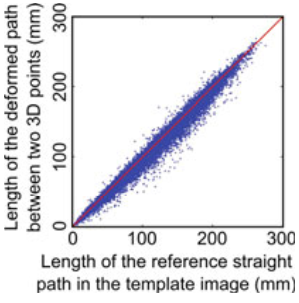
\includegraphics[width=1.0\linewidth]{img/fig4a.png}
                図a) FFDinit
            \end{column}
            \begin{column}[T]{0.32\textwidth} % 右:40%
                \centering
                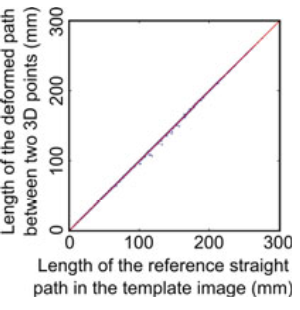
\includegraphics[width=1.0\linewidth]{img/fig4b.png}
                図b) FFDref
            \end{column}
            \begin{column}[T]{0.32\linewidth} % 右:40%
                \centering
                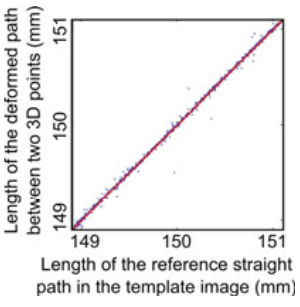
\includegraphics[width=1.0\linewidth]{img/fig4c.png}
                図c) FFDrefの拡大図
            \end{column}
        \end{columns}
        図1 非伸張性の証明
     \end{block}
  \end{frame}
 %    \begin{frame}{スライドタイトル}
 %     \begin{block}{}
 %         \centering
 %        \begin{columns}[onlytextwidth]
 %            \begin{column}[T]{0.32\textwidth} % 左:60%
 %                \centering
 %                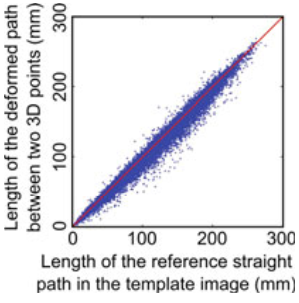
\includegraphics[width=1.0\linewidth]{img/fig4a.png}
 %                FFDinit
 %            \end{column}
 %            \begin{column}[T]{0.32\textwidth} % 右:40%
 %                \centering
 %                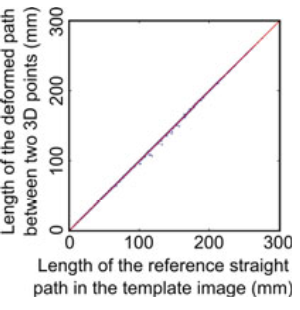
\includegraphics[width=1.0\linewidth]{img/fig4b.png}
 %                FFDref
 %            \end{column}
 %            \begin{column}[T]{0.32\linewidth} % 右:40%
 %                \centering
 %                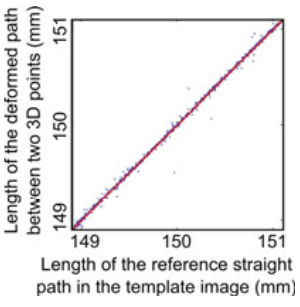
\includegraphics[width=1.0\linewidth]{img/fig4c.png}
 %                FFDrefの拡大図
 %            \end{column}
 %        \end{columns}
 %        非伸張性の証明
 %     \end{block}
 %    \end{frame}
    \begin{frame}{ガウス曲率}
        \begin{itemize}
            \item 表面における2方向の主曲率の積:ガウス曲率
            \item ガウス曲率が0の時,その面は非伸縮
            \item 再構成した表面上の点の10,000組のガウス曲率を計算
        \end{itemize}
\begin{table}[htb]
  \caption{ガウス曲率による提案手法の非伸長性評価}
  \centering
  {\tiny
  \begin{tabular}{|r|r|r|r|r|r|} \hline
      & Mean & Std. deviation & Median & Mininum & Maximum \\ \hline
      FFDinit& $4.9458\times10^{-4}$ & 0.0875 & $9.7302\times10^{-5}$ & $7.5122\times10^{-14}$ & 258.2379 \\ \hline
      FFDref& $5.0046\times1-^{-6}$ & $7.1320\times10^{-4}$ & $1.7333\times10^{-6}$ & $2.2325\times10^{-14}$ & 1.5199 \\ \hline
  \end{tabular}
  }
  \label{table3}
\end{table}
    \end{frame}
  \begin{frame}{参考文献}
    \bibliographystyle{sieicej}
    \bibliography{library}%bibTexのファイル名
\end{frame}
\end{document}
